\documentclass[12pt]{article}

\RequirePackage{../macros/mumie}

\def\t#1{\texttt{#1}}

\begin{document}

%%%%%%%%%  START Titelseite %%%%%%%%%
\thispagestyle{empty}

\vspace*{1cm}%

%\font\authorfont=cmss10 scaled 1440\relax
%\font\titlefont=ccr10 scaled 3456\relax

\begin{center}
\phantom.
\vspace*{5cm}

\texttt{\Huge mumie} \textsf{\Huge Style Guide}
\bigskip

\styletitle{Data and Source File Naming Conventions}
\phantom.
\vspace*{3cm}

\ifx\pdfoutput\undefined
  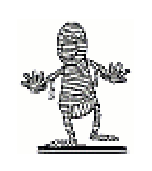
\epsfig{file=../macros/mumie_klein.ps,width=2cm,angle=0}
\else
  
\includegraphics[width=2cm,angle=0]{../macros/mumie_klein.pdf}
\fi
\vspace*{3cm}

\begin{tabular}{ll}
\textsf{Maintainer:}& Dominik Eberlein\\
\textsf{Datum:}& \verb+$Date: 2004/01/28 19:36:53 $+\\                  % Wird vom cvs eingetragen
\textsf{CVS-Version:}& \verb+$Revision: 1.3 $+\\                % Wird vom cvs eingetragen
\textsf{CVS-Source:}&\verb+$Source: /net/mumie/cvs/styles/naming/main.tex,v $+\\ % Wird vom cvs eingetragen
\end{tabular}
\end{center}

\clearpage
%%%%%%%%% END Titelseite %%%%%%%%% 

\tableofcontents
\eject

\section{Einf�hrung}

Im folgenden steht~$\t x_\t i$ jeweils f�r genau ein Zeichen. Soweit
nicht explizit etwas anderes vereinbart ist, kann es sich um eines der
Zeichen~\t a bis~\t z und~\t0 bis~\t9 handeln.

\section{Konventionen zur Bezeichnung der Kurse, Module, Elemente und Subelemente im Lehrmodul}

Die folgenden Konventionen legen die Bezeichnungen von Kursen, Modulen, Elementen und Subelementen im gesamten
\mumie-Projekt fest.

\subsection{Kurse}

Kurse werden wie folgt bezeichnet:
\[\t l\t x_\t1 \t x_\t2 \t x_\t3 \]

Dabei stehen~$\t l$ f�r Lehrmodul und~$\t x_\t1 \t x_\t2 \t x_\t3$ f�r die eindeutige
Bezeichnung des Kurses ($\to$ Modulliste).

\emph{Beispiel:} Kurs Lineare Algebra: $\t l\t l\t i\t a$

\subsection{Module}

Die Benennung eines Moduls im Kurs~$\t x_\t1 \t x_\t2 \t x_\t3$ ist so:
\[\t l\t x_\t1 \t x_\t2 \t x_\t3 \t x_\t4 \t x_\t5 \t x_\t6 \]

Dabei ist~$ \t x_\t4 \t x_\t5 \t x_\t6$ die eindeutige Modulnummer ($\to$ Modulliste).

\emph{Beispiel:} Modul Gau� im Kurs Lineare Algebra:  $\t l\t l\t i\t a\t0\t0\t8$

\subsection{Elemente und Subelemente}

Die Bezugnahme auf ein Element oder Subelement im Modul~$\t l\t x_\t1 \t x_\t2 \t x_\t3 \t x_\t4 \t x_\t5 \t x_\t6$
erfolgt so:

\[\t l\t x_\t1 \t x_\t2 \t x_\t3 \t x_\t4 \t x_\t5 \t x_\t6 \t x_\t7 \t x_\t8 \t x_\t9 \]

Hier gibt~$\t x_7$ den Element- oder Subelementtyp an. Folgende M�glichkeiten gibt es:

\begin{tabular}{ll}
Motivation:&\t m\\
Theorem:&\t t\\
Definition:&\t d\\
Algorithmus:&\t a\\
Anwendung:&\t l\\
Eigenschaften:&\t p\\
\end{tabular}\qquad
\begin{tabular}{ll}
Beweis:&\t f\\
Visualisierung:&\t v\\
Beispiel:&\t e\\
Bemerkung:&\t r\\
Historie:&\t h\\
\end{tabular}

Die letzten beiden Zeichen~$\t x_\t8\t x_\t9$ sind eine (im Modul eindeutige) Identifikationsnummer f�r diesen Elementtyp.

\emph{Beispiele:} 

Motivation im Modul Gau�, Kurs Lineare Algebra: $\t l\t l\t i\t a\t0\t0\t8\t m\t0\t0$

1.~Satz im Modul Gau�, Kurs Lineare Algebra: $\t l\t l\t i\t a\t0\t0\t8\t t\t0\t0$

2.~Satz im Modul Gau�, Kurs Lineare Algebra: $\t l\t l\t i\t a\t0\t0\t8\t t\t0\t1$

\section{Konventionen f�r die Bennenung und Hierachie von CVS-verwalteten Projektteilen}

\subsection{Modul \mumie}

Im Modul~\mumie sind die gesamten Quelldateien f�r das Endprodukt
enthalten. Die Verzeichnisstruktur ist wie folgt:

\begin{tabbing}
\t{admin/}\=$\t x_\t1\t x_\t2\t x_\t3/$\=$\t x_\t1\t x_\t2\t x_\t3/$\qquad\=\kill
\t{admin/}\>\>\>verschiedene Tools zur Administration des Moduls~\mumie\\
\t{l/}\>\>\>Dateien/Verzeichnisse zum Lehrmodul\\
\>\t{lia/}\>\>Dateien/Verzeichnisse zum Kurs ``Lineare Algebra''\\
\>$\vdots$\\
\>$\t x_\t1\t x_\t2\t x_\t3/$\>\>Dateien/Verzeichnisse zu Kurs $\t x_\t1\t x_\t2\t x_\t3$\\
\>\>\t{000/}\>Dateien zum Modul~\t{000}\\
\>\>$\vdots$\\
\>\>$\t x_\t4\t x_\t5\t x_\t5/$\>Dateien zum Modul~$\t x_\t4\t x_\t5\t x_\t6$\\
\end{tabbing}

In dem Verzeichnis~\t l/$\t x_\t1\t x_\t2\t x_\t3/$$\t x_\t1\t x_\t2\t
x_\t3/$ befinden sich also die Dateien zum Modul 
$\t l\t x_\t1 \t x_\t2 \t x_\t3 \t x_\t4 \t x_\t5 \t x_\t6$. Die Dateienamen sind wie
folgt aufgabaut:

\begin{tabular}{ll}
$\t l\t x_\t1 \t x_\t2 \t x_\t3 \t x_\t4 \t x_\t5 \t
x_\t6\t{-struct.xml}$&Strukturdatei f�r das Modul\\ $\t l\t x_\t1 \t
x_\t2 \t x_\t3 \t x_\t4 \t x_\t5 \t x_\t6\t x_\t7\t x_\t8\t
x_\t9\t{.tex}$&\TeX-Source f�r das (Sub-)Element~$\t x_\t7\t x_\t8\t
x_\t9$ im Modul\\ $\t l\t x_\t1 \t x_\t2 \t x_\t3 \t x_\t4 \t x_\t5 \t
x_\t6\t x_\t7\t x_\t8\t x_\t9\t{-xxx.xxx}$& weitere Dateien zu dem
Element oder Subelement (todo)\\
\end{tabular}

\end{document}
